\begin{figure*}[t]
  \centering
  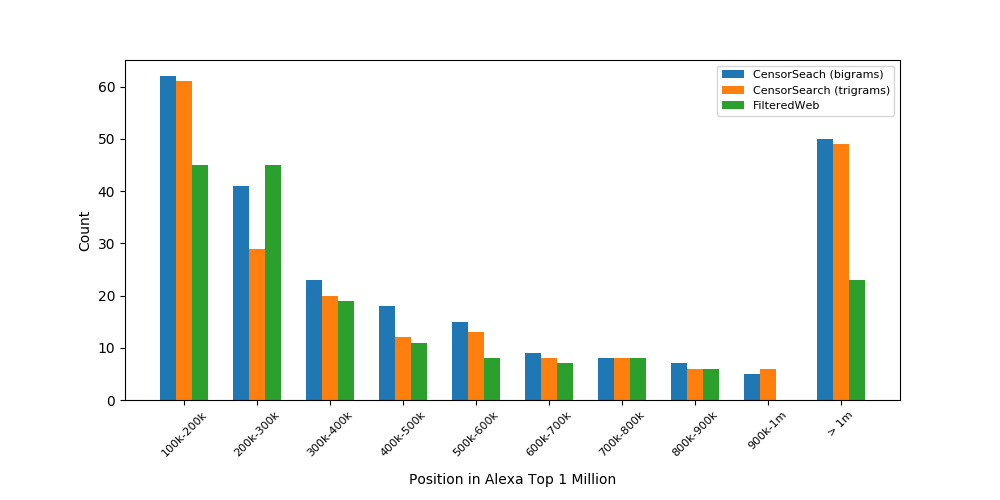
\includegraphics[scale=0.6]{figures/alexa}
  \caption{\label{alexa}Ranking of censored websites on Alexa Top 1 Million.}
\end{figure*}

\section{Results}
We reached several key insights from performing our
evaluations. First, we were able to discover hundreds of
censored websites that are not present on existing block
lists. Furthermore, we noticed that many websites on our block list
receive very little traffic. Lastly, we found that by using
politically-charged phrases as search terms, we were able to find a
disproportionately large amount of censored websites. The rest of this
section discusses the main findings in depth.

\subsection{Existing blocklists are incomplete}
\textit{By using natural-language processing on Chinese web pages, we
were able to discover hundreds of censored websites that are not
present on the Citizen Lab block list--the standard for censorship
measurements--and FilteredWeb's block list~\cite{darer2017filteredweb,
citizenlab:block}}. Furthermore, only 3 of the top 50 censored domains
that appeared in our search results are in the top 50 censored domains
found by FilteredWeb. Figure~\ref{top-domains} breaks down the URL
count for the top 25 censored domains that we discovered. These
websites seem to mainly cover Chinese human rights issues, news,
censorship circumvention, and more.

For instance, \texttt{wiki.zhtube.com} appears to be a Chinese
Wikipedia mirror. The web page for \texttt{zhtube.com} seems to be the
default page for a Chinese LNMP (Linux, NginX MySQL, PhP) installation
on a virtual private server~\cite{lnmp}. We found over 3000 URLs in
our dataset that point to this website, which may suggest that Chinese
websites are trying to circumvent the on-and-off censorship of
Wikipedia in China~\cite{wikipedia-china}. Furthermore,
\texttt{blog.boxun.com} is a United States-based outlet for Chinese
news that relies heavily on anonymous submissions. The owners of the
website note that ``Boxun often reports news that authorities do not
tell the public, such as outbreaks of diseases, human rights
violations, corruption scandals and
disasters''~\cite{boxun-about}. \textit{Thus, by building on the
approach of FilteredWeb, we were able to produce a qualitatively
different block list}. We recommend putting these two block lists
together to create a single block list that is both wide in scope and
large in size.

Intuitively, we were able to find hundreds of qualitatively
different censored domains than those found by FilteredWeb because
we could extract Chinese-specific topics from web pages. We were able
to do so by using TF-IDF with a Chinese corpus to rank the
``uniqueness'' of Chinese phrases that appeared on a given
web page. For example, the trigram
\begin{CJK*}{UTF8}{gbsn}仅 限于 书面\end{CJK*} (``only written'') was poorly ranked on
\texttt{tiananmenmother.org}--a Chinese democratic activist group--
because although it appears frequently, it's a common phrase in
Chinese, according to the Chinese corpus on
PhraseFinder~\cite{phrasefinder}. On the other hand, the
trigram \begin{CJK*}{UTF8}{gbsn}自由 亚洲 电台\end{CJK*} (``Radio Free
Asia'') was highly ranked because it didn't appear frequently, and
it's an uncommon phrase in Chinese. It should also be noted that Radio
Free Asia is a broadcasting corporation whose stated mission is to
``provide accurate and timely news and information to Asian countries
whose governments prohibit access to a free
press''~\cite{rfa:about}. Thus, by scoring Chinese phrases with TF-IDF
against a Chinese corpus, we were able to determine which phrases are
``content-rich'' on a given web page.

\begin{table}[b]
  \begin{center}
    \scalebox{0.80}{
    \begin{tabular}{ | l | r | r | r | }
      \hline
      Phrase length & Domains & Domains w/o Alexa Top 1000 \\ \hline
      Unigrams      & 1029    & 765 \\
      Bigrams       & 970     & 655 \\
      Trigrams      & 975     & 629 \\
      Total         & 1756    & \textbf{1125} \\
      \hline
    \end{tabular}}
  \end{center}
\caption{\label{breakdown} Total number of censored domains discovered.}
\end{table}

\subsection{China blocks many unpopular websites}
Figure~\ref{alexa} shows the ranking of the websites we discovered on
the Alexa Top 1,000,000. Notably, many of the websites we discovered
are spread throughout the tail of the list, and some of the websites
are not even on the list at all. \textit{Given that the top 100,000 websites
likely receive the vast majority of traffic on the Internet, we can
infer that censors in China are not just interested in blocking
``big-name'', popular websites.} They are actively seeking out websites
of \textit{any size} that contain ``sensitive'' content. We also
discovered a number of websites that fall outside the Alexa Top
1,000,000 altogether. Without the use of an automated system that can
discover censored websites, it's unlikely that the public would even
be aware that these websites are blocked.

\begin{figure}[t]
  \centering
  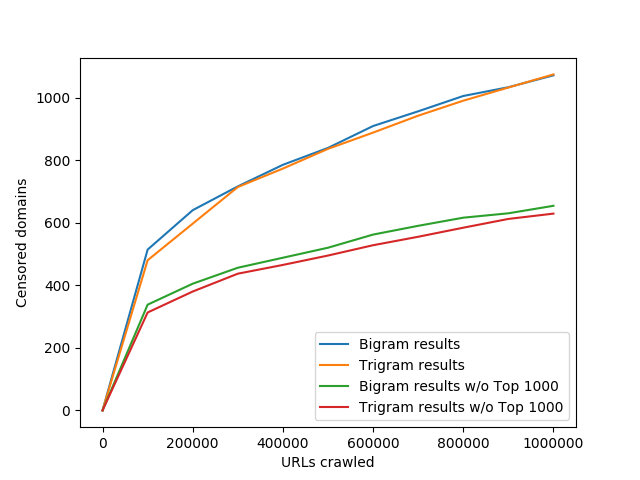
\includegraphics[scale=0.5]{figures/urls-crawled}
  \caption{\label{censored-vs-urls} Censored domains discovered over unique URLs crawled. }
\end{figure}

\begin{table}[b]
  \begin{center}
    \scalebox{0.9}{
      \begin{tabular}{ l | l | c }
        Chinese & English & Censored domains \\ \hline
        \begin{CJK*}{UTF8}{gbsn}王歧山\end{CJK*} & Wang Qishan & 74\% \\
        \begin{CJK*}{UTF8}{gbsn}李洪志\end{CJK*} & Li Hongzhi & 64\% \\
        \begin{CJK*}{UTF8}{gbsn}郭伯雄\end{CJK*} & Guo Boxiong & 62\% \\
        \begin{CJK*}{UTF8}{gbsn}胡锦涛\end{CJK*} & Hu Jintao & 56\% \\
        \begin{CJK*}{UTF8}{gbsn}胡平\end{CJK*}  & Hu Ping & 54\% \\
        \begin{CJK*}{UTF8}{gbsn}Morty\end{CJK*} & Morty & 52\% \\
        \begin{CJK*}{UTF8}{gbsn}命案\end{CJK*}  & Homicide & 52\% \\
        \begin{CJK*}{UTF8}{gbsn}特首\end{CJK*}  & Chief executive & 52\% \\
        \begin{CJK*}{UTF8}{gbsn}Vimeo\end{CJK*} & Vimeo & 50\% \\
        \begin{CJK*}{UTF8}{gbsn}中情局\end{CJK*} & CIA & 50\% \\
      \end{tabular}}
  \end{center}
  \caption{\label{effective-unigrams}Sample of unigrams with
    significant blockrates}
\end{table}

Table \ref{breakdown} shows the breakdown of how many censored
websites we discovered. By using unigrams, we were able to discover
765 domains that are not on any publicly available block list. By
using bigrams, we were able to discover 655 censored domains. Lastly,
by using trigrams, we were able to discover 629 censored domains. In
total, we discovered 1125 censored domains, none of which are on the
Alexa Top 1000~\cite{alexa:top1000}. Each of these evaluations were
performed with 1,000,000 unique URLs, consistent with the methodology
of FilteredWeb~\cite{darer2017filteredweb}. Figure
\ref{censored-vs-urls} shows how many censored domains we discovered
as a function of unique URLs crawled for each evaluation.

\begin{table*}[t]
  \begin{center}
    \scalebox{0.9}{
      \begin{tabular}{ l | l | c }
        Chinese & English & Censored domains \\ \hline
        \begin{CJK*}{UTF8}{gbsn}中共\end{CJK*} \begin{CJK*}{UTF8}{gbsn}威胁\end{CJK*} & Chinese Communists threaten & 50\% \\
        \begin{CJK*}{UTF8}{gbsn}声明的\end{CJK*} \begin{CJK*}{UTF8}{gbsn}反共产主义\end{CJK*} & Declared anti-communist & 44\% \\
        \begin{CJK*}{UTF8}{gbsn}中国共\end{CJK*} \begin{CJK*}{UTF8}{gbsn}产党的公共安全\end{CJK*} & Public security of the CPC & 42\% \\
        \begin{CJK*}{UTF8}{gbsn}北京\end{CJK*} \begin{CJK*}{UTF8}{gbsn}清洁\end{CJK*} & Beijing clean-up & 40\% \\
        \begin{CJK*}{UTF8}{gbsn}江泽民\end{CJK*} \begin{CJK*}{UTF8}{gbsn}胡锦涛\end{CJK*} & Jiang Zemin Hu Jintao & 40\% \\
        \begin{CJK*}{UTF8}{gbsn}迫害\end{CJK*} \begin{CJK*}{UTF8}{gbsn}活动\end{CJK*} & Persecution
                                                     activities & 40\% \\
        \begin{CJK*}{UTF8}{gbsn}官员\end{CJK*} \begin{CJK*}{UTF8}{gbsn}呼吁\end{CJK*} & Officials called on & 36\% \\
        \begin{CJK*}{UTF8}{gbsn}重的\end{CJK*} \begin{CJK*}{UTF8}{gbsn}公民\end{CJK*} & Heavy Citizen & 36\% \\
        \begin{CJK*}{UTF8}{gbsn}非法\end{CJK*} \begin{CJK*}{UTF8}{gbsn}拘留\end{CJK*} & Illegal detention
                          & 36\% \\
        \begin{CJK*}{UTF8}{gbsn}不同\end{CJK*} \begin{CJK*}{UTF8}{gbsn}的民主\end{CJK*} & Different Democratic & 34\% \\
      \end{tabular}}
  \end{center}
  \caption{\label{effective-bigrams}Sample of bigrams with significant
    block rates}
\end{table*}

\begin{table*}[t]
  \begin{center}
    \scalebox{0.9}{
      \begin{tabular}{ l | l | c }
        Chinese & English & Censored domains \\ \hline
        \begin{CJK*}{UTF8}{gbsn}北戴\end{CJK*} \begin{CJK*}{UTF8}{gbsn}河\end{CJK*} \begin{CJK*}{UTF8}{gbsn}会议\end{CJK*} & BEIDAIHE meeting & 54\% \\
        \begin{CJK*}{UTF8}{gbsn}中国\end{CJK*} \begin{CJK*}{UTF8}{gbsn}共产党\end{CJK*} \begin{CJK*}{UTF8}{gbsn}的宗教政策\end{CJK*} & The Chinese Communist Party's religious policy & 42\% \\
        \begin{CJK*}{UTF8}{gbsn}采取\end{CJK*} \begin{CJK*}{UTF8}{gbsn}暴力\end{CJK*} \begin{CJK*}{UTF8}{gbsn}镇压\end{CJK*} & To take a violent crackdown & 38\% \\
        \begin{CJK*}{UTF8}{gbsn}香港\end{CJK*} \begin{CJK*}{UTF8}{gbsn}政\end{CJK*} \begin{CJK*}{UTF8}{gbsn}治\end{CJK*} & Hong Kong Politics & 34\% \\
        \begin{CJK*}{UTF8}{gbsn}欧洲\end{CJK*} \begin{CJK*}{UTF8}{gbsn}议会\end{CJK*} \begin{CJK*}{UTF8}{gbsn}决议\end{CJK*} & European Parliament Resolution & 32\% \\
        \begin{CJK*}{UTF8}{gbsn}新\end{CJK*} \begin{CJK*}{UTF8}{gbsn}唐\end{CJK*} \begin{CJK*}{UTF8}{gbsn}王朝\end{CJK*} & New Tang Dynasty & 32\% \\
        \begin{CJK*}{UTF8}{gbsn}恐怖\end{CJK*} \begin{CJK*}{UTF8}{gbsn}事件\end{CJK*} \begin{CJK*}{UTF8}{gbsn}。\end{CJK*} & A terrorist event. & 32\% \\
        \begin{CJK*}{UTF8}{gbsn}天安\end{CJK*} \begin{CJK*}{UTF8}{gbsn}门广\end{CJK*} \begin{CJK*}{UTF8}{gbsn}场示威\end{CJK*} & Tienanmen Square Demonstrations & 32\% \\
        \begin{CJK*}{UTF8}{gbsn}敦促\end{CJK*} \begin{CJK*}{UTF8}{gbsn}美国\end{CJK*} \begin{CJK*}{UTF8}{gbsn}政府\end{CJK*} & Urging the US government & 32\% \\
        \begin{CJK*}{UTF8}{gbsn}1989\end{CJK*} \begin{CJK*}{UTF8}{gbsn}民主\end{CJK*} \begin{CJK*}{UTF8}{gbsn}运动\end{CJK*} & 1989 democracy movement & 30\% \\
      \end{tabular}}
  \end{center}
  \caption{\label{effective-trigrams}Sample of trigrams with
    significant blockrates}
\end{table*}

\subsection{Political phrases are highly effective}
\label{phrases-eval}

We also wanted to see if there is a correlation between the
presence of certain phrases and whether or not a given website is
censored, even if we have no ground truth.  For example, if we make a search
for \begin{CJK*}{UTF8}{gbsn}中国侵犯人权\end{CJK*} (Chinese human
rights violation) and find that a particular search result is
censored, then we cannot be certain whether the presence of that phrase
\textit{caused} the website to be blocked. Even if we assume 
that a censor is manually combing through search engines to find
sensitive websites, the website could have been blocked because it
contained totally different content.

Nevertheless, there seems to be some correlation for certain
phrases. Table~\ref{effective-unigrams} shows a sample of unigrams
that returned the most number of unique filtered domains from
Bing. For example, the top four unigrams--Wang Qishan, Li Hongzhi, Guo
Boxiong, and Hu Jintao--are the names of controversial figures in
Chinese history. Li Hongzhi is the leader of the Falun Gong spiritual
movement, whose practitioners have been subject to persecution and
censorship by the Chinese government since
1999~\cite{freedomhouse:falun}. Similarly, Guo Boxiong is a former top
official of the Chinese military that was sentenced to life in
prison in 2016 for accepting bribes, according to the Chinese
government~\cite{guardian:guo}. Thus, if a Chinese website discusses
these people, the website may become censored for containing
``sensitive'' content.

There are also bigrams that correlate with a large percentage of
censored domains, but they are more explicitly political than the
unigrams. Table~\ref{effective-bigrams} shows this result. First, most
of the bigrams refer to the Chinese Communist Party in some
way. Phrases such as \begin{CJK*}{UTF8}{gbsn}中共的威胁\end{CJK*}
(Chinese Communists threaten), \begin{CJK*}{UTF8}{gbsn}江泽民胡锦
涛\end{CJK*} (Jiang Zemin Hu Jintao), and \begin{CJK*}{UTF8}{gbsn}中国
共产党的治安\end{CJK*} (Public security of the CPC) do not necessarily
convey sensitive information, but they nonetheless refer to the
government of China. On the other hand, some phrases clearly refer to
political dissent, such as \begin{CJK*}{UTF8}{gbsn}官员呼吁\end{CJK*}
(Officials called on), \begin{CJK*}{UTF8}{gbsn}迫害活动\end{CJK*}
(Persecution activities), \begin{CJK*}{UTF8}{gbsn}非法拘留\end{CJK*}
(Illegal detention), and \begin{CJK*}{UTF8}{gbsn}宣称反共\end{CJK*}
(Declared anti-communist).

We see a similar result with trigrams, as shown by
Table~\ref{effective-trigrams}. Phrases that stand out
include \begin{CJK*}{UTF8}{gbsn}中国共产党的宗教政策\end{CJK*} (The
Chinese Communist Party's religious policy), \begin{CJK*}{UTF8}{gbsn}
天安门广场示威\end{CJK*} (Tienanmen Square
demonstrations), \begin{CJK*}{UTF8}{gbsn}1989年民主运动\end{CJK*}
(1989 democracy movement), and \begin{CJK*}{UTF8}{gbsn}采取暴力镇
压\end{CJK*} (To take a violent crackdown). Interestingly, we also see
that discussion of China's religious policy, the ``New Tang
Dynasty''--a religious radio broadcast located in the United States--,
and European Union legislation may also be considered sensitive
content.~\cite{china-religion}. \textit{Together, these results
suggest that references to collective political dissent are highly
likely to be censored}. This is consistent with the findings of King
et al.~\cite{king2013censorship}.
